%% Section 2 — Conceptual Background
\section{Conceptual Background}
\label{sec:background}

\subsection{The literature and its limits}

The existing literature on data centers is, in aggregate, large and growing. But its organisation into disconnected silos is not incidental to the phenomena it studies — it is a product of the disciplinary assumptions each silo imports. The technical efficiency literature treats data centers as engineering optimisation problems: cooling infrastructure, power usage effectiveness ratios, hardware lifecycle management. The environmental impact literature treats them as emissions sources to be measured and, where possible, reduced. The socio-political literature — thinner, more dispersed, and largely invisible to the other two — treats them as sites of ethnographic interest, following \citet{blum2012tubes}, \citet{holt2015vonderau}, and \citet{vonderau2019storing} in attending to the material, political, and cultural dimensions of infrastructure that the engineering literature abstracts away.

None of these literatures possesses the conceptual tools to account for data centers as a \textit{systemic} phenomenon: an infrastructure regime being constituted through the ongoing interactions of heterogeneous actors across multiple scales, involving feedback loops between technological change, investment structures, planning systems, community mobilisation, and regulatory response. This is precisely the terrain for which the Multi-Level Perspective \citep{geels2002technological}, Technological Innovation Systems, and sociotechnical regime analysis were developed — and it is, as the bibliometric audit establishes, terrain they have not yet entered.

\subsection{Datacentering as a concept}

We propose \textit{datacentering} as a conceptual reframing adequate to this terrain. The choice of a gerund is deliberate. Where ``data center'' names a technical object with fixed properties, ``datacentering'' names a \textit{process}: the ongoing, contested, socio-material practice of assembling, operating, expanding, and reproducing digital infrastructure in particular places, by particular actors, for particular purposes, under particular conditions of governance and resistance. The concept draws on two theoretical lineages.

The first is \citeauthor{orlikowski2007sociomaterial}'s \citeyear{orlikowski2007sociomaterial} account of sociomaterial practice: the claim that technology and social practice are constitutively entangled rather than separately analysable. A data center is not a technical substrate onto which social processes are then layered; the servers, the cooling towers, the power contracts, the planning permissions, the community objections, and the financial instruments are all co-constitutive elements of the same socio-material assemblage. To study the assemblage, one must be able to reach all its elements — hence the multimodal agenda this paper develops.

The second lineage is the sociology of sociotechnical imaginaries \citep{jasanoff2015dreamscapes}: the claim that the representations through which actors understand and communicate about technology are not mere descriptions of material facts but co-producers of those facts. ``The cloud'' is the paradigm case. It is an imaginary that naturalises infrastructure, decouples computation from territory, and positions data center campuses as nodes in a universal technical commons rather than as large-scale industrial land uses embedded in specific watersheds, power grids, and communities. The imaginary does not merely describe the infrastructure; it shapes how planning systems respond to it, how investors price it, how communities mobilise against it, and how operators justify their presence to municipal authorities. Datacentering is, in part, the continuous work of maintaining and contesting this imaginary.

\subsection{Complex adaptive systems as a sensemaking lens}

We draw on complex adaptive systems (CAS) thinking not as a formal operationalised framework but as a sensemaking lens: a way of apprehending the systemic character of the phenomena before deciding how to study them. \citet{phillips2019complex} provide the most directly applicable treatment, proposing a CAS-based methodology for ecosystem research organised around three dimensions: \textit{conceptual} (boundaries, perspectives, and imaginaries: how we think about the system), \textit{structural} (hierarchy, relationships, and actor constellations: what we know about the system), and \textit{temporal} (dynamics and co-evolution: how the system changes over time).

Applied to datacentering, the CAS lens immediately surfaces features — illustrated in \Cref{fig:constellation} — that that the existing literature misses. The actor constellation is genuinely heterogeneous: hyperscale operators, colocation providers, REIT asset managers, pension fund investors, cloud computing tenants, municipal authorities, planning inspectors, community campaign groups, environmental regulators, energy grid operators, and water utilities are all constitutive actors in the assemblage — not merely context for it. Their interactions are nonlinear: the same intensity of community contestation produces a planning moratorium in Amsterdam and no discernible governance response in Northern Virginia, a difference not explicable by the strength of the signal but by the structural properties of the system receiving it. And the outcomes are emergent: no single actor in the Loudoun County data center market planned for it to become the highest-concentration cluster in the world; that outcome is the emergent product of thousands of individual location, investment, and planning decisions interacting under conditions no single actor controlled.

\begin{fullwidth}
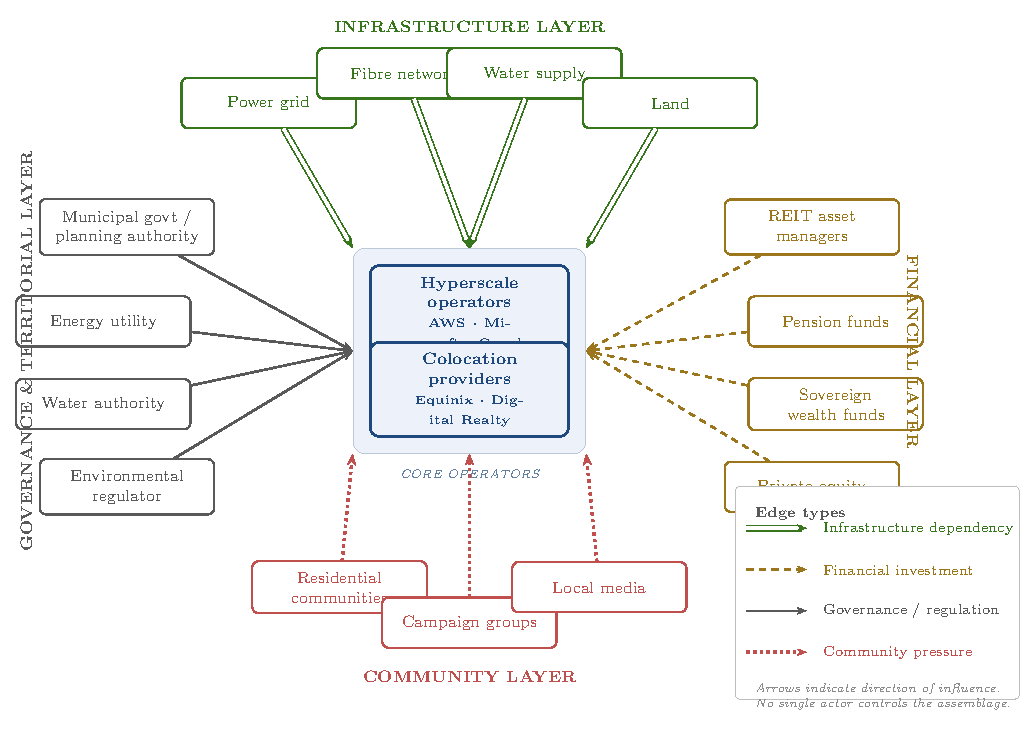
\includegraphics[width=\linewidth]{figures/actor-constellation}
\vspace{0.4em}
\captionof{figure}{The multi-actor constellation of a data center assemblage. No single actor controls the system; outcomes are emergent products of interactions across corporate, financial, governance, community, and infrastructure layers.\label{fig:constellation}}
\end{fullwidth}

The research agenda this paper develops is structured around the first two CAS dimensions — conceptual and structural — with the temporal dimension introduced as the dynamic layer through which contestation and regime response become legible. The CAS framing motivates not only the multimodal methodology but also the open cartography: if the phenomena are genuinely CAS-like, then the knowledge required to map them is itself distributed across actors, jurisdictions, and disciplines in ways that make any single-researcher or single-team approach structurally inadequate. The open research infrastructure is the methodological response to the complexity of the object.
